\chapter{Diseño}
En este capítulo se abordará el diseño del sistema. Para ello, en primer
lugar, se va a realizar el diseño de la base de datos con el modelo
entidad-relación, el paso a tablas y la normalización. En segundo lugar,
se realizará el diseño de las interfaces de usuario. Por se hablará del
diseño de la arquitectura del sistema.

\section{Diseño de base de datos}
En esta sección vamos a abordar el diseño de la base de datos.
Comenzaremos con el modelo entidad-relación y terminaremos con el paso a
tablas y la normalización.

\subsection{Modelo Entidad-Relación}
En la figura \ref{fig:e-r} se muestra el modelo entidad-relación de la base de
datos. En dicho modelo se encuentran las entidades con sus atributos y las
relaciones entre ellas.

Vemos que la entidad \texttt{Artista} hereda de la entidad \texttt{Usuario}.
Esto se hace para poder relacionar la entidad \texttt{Artista} con la entidad
\texttt{ObraDeArte} a través de la relación \texttt{Tiene} y que sea independiente
de la entidad \texttt{Usuario} ya que solamente los usuarios que sean artistas
podrán tener obras de arte.

La entidad \texttt{Usuario} tiene una relación \texttt{Realiza} con la entidad
\texttt{Valoración} indicando que un usuario puede realizar varias valoraciones.
A su vez la entidad \texttt{Valoración} tiene una relación \texttt{Pertenece} con
la entidad \texttt{ObraDeArte} indicando que una valoración pertenece a una obra
de arte.

\begin{figure}[H]
  \centering
  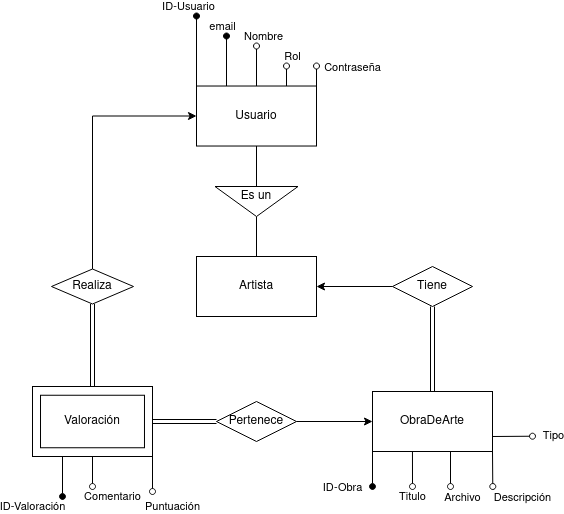
\includegraphics[width=\textwidth]{diagramas/e-r}
  \caption{Modelo entidad-relación}
  \label{fig:e-r}
\end{figure}

\subsection{Paso a tablas}
A continuación vamos a realizar el paso a tablas del modelo entidad-relación. Para
ello haremos las tablas primero de las entidades fuertes, luego entidades débiles
y por último las relaciones.

\begin{enumerate}
    \item \[ \texttt{Usuario}(\underline{ID-Usuario}_{CP}, \underline{Email}_{CC}, Nombre, Contraseña) \]
    \item \[ \texttt{Artista}(\underline{ID-Usuario}_{CP}^{CE1}) \]
    \item \[ \texttt{ObraDeArte}(\underline{ID-Obra}_{CP}, Titulo, Descripción, Tipo, Archivo) \]
    \item \[ \texttt{Valoración}(\underline{ID-Valoración}_{CP}, Puntuación, Comentario) \]
    \item \[ \texttt{Tiene}(\underline{ID-Obra}_{CP}^{CE3}, ID-Usuario^{CE2}) \]
    \item \[ \texttt{Pertenece}(\underline{ID-Valoración}_{CP}^{CE4}, ID-Obra^{CE3}) \]
    \item \[ \texttt{Realiza}(\underline{ID-Valoración}_{CP}^{CE4}, ID-Usuario^{CE1}) \]
\end{enumerate}

\vspace{1cm}
Ahora se va a proceder a fusionar las tablas que sean posibles. Además,
dado que la tabla \texttt{Artista} no tiene atributos propios y solamente tiene
una clave externa que es clave primaria en la tabla \texttt{Usuario} (que es la
tabla padre) , se puede fusionar con dicha tabla, añadiendo a esta una columna
que indique si el usuario es artista o no, será el atributo \texttt{Rol}.

\begin{enumerate}
    \item \[ \texttt{Usuario}(\underline{ID-Usuario}_{CP}, \underline{Email}_{CC}, Nombre, Contraseña, Rol) \]
    \item \[ \texttt{ObraDeArte}(\underline{ID-Obra}_{CP}, Titulo, Descripción, Tipo, Archivo, ID-Usuario^{CE1}) \]
    \item \[ \texttt{Valoración}(\underline{ID-Valoración}_{CP}, Puntuación, Comentario, ID-Obra^{CE2}, ID-Usuario^{CE1}) \]
\end{enumerate}

\subsection{Normalización}
Dado que todos los atributos de las tablas están en 1FN, vamos a proceder a
normalizar las tablas a 2FN y 3FN.

\subsubsection{2FN}
Para que una tabla esté en 2FN debe estar en 1FN y además todos los atributos
que no pertenezcan a la clave primaria deben depender de esta.

En nuestro caso, todas las tablas están en 1FN y además todos los atributos
dependen de la clave primaria, por lo que todas las tablas están en 2FN.

\subsubsection{3FN}
Para que una tabla esté en 3FN debe estar en 2FN y además todos los atributos
que no pertenezcan a la clave primaria deben depender únicamente de dicha
clave primaria y no de otros atributos.

En nuestro caso, todas las tablas están en 2FN y además todos los atributos
dependen de la clave primaria y no de otros atributos no-clave, por lo que
todas las tablas están en 3FN.

\section{Diseño de interfaces de usuario}

\section{Diseño de la arquitectura del sistema}
A continuación se va a explicar la arquitecura del sistema utilizada.
Para la creación de la aplicación web se va a utilizar el patrón
Modelo-Vista-Controlador (MVC).

\subsection{Modelo-Vista-Controlador}
Este patrón de arquitectura se basa en separar la lógica de la aplicación
en tres partes:

\begin{itemize}
    \item \textbf{Modelo}: El modelo representa la información con la que trabaja
    la aplicación. En el caso de la aplicación que vamos a desarrollar, el modelo
    será la base de datos y las funciones del backend que se encarguen de gestionarla.
    \item \textbf{Vista}: La vista es la parte encargada de mostrar la información
    al usuario y permitir que este interactúe con la aplicación. En el caso de la
    aplicación que vamos a desarrollar, la vista será la parte del frontend.
    \item \textbf{Controlador}: El controlador es el encargado de gestionar las
    peticiones del usuario y realizar las acciones correspondientes. Es el enlace
    entre la vista y el modelo. En nuestra aplicación el controlador será la parte
    del backend que se encargue de gestionar las peticiones provenientes del frontend
    y a través de una serie de funciones \textit{getters} y \textit{setters} se
    pedirá y modificará la información del modelo.
\end{itemize}

En la figura \ref{fig:mvc} se muestra un diagrama de la arquitectura MVC de la
aplicación.

\begin{figure}[H]
  \centering
  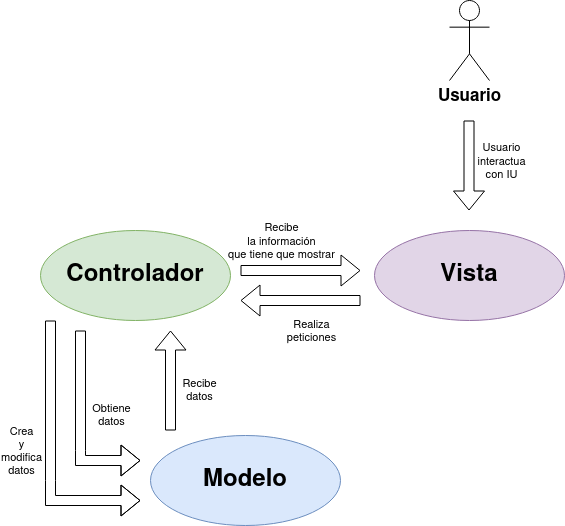
\includegraphics[width=\textwidth]{diagramas/mvc}
  \caption{Modelo-Vista-Controlador}
  \label{fig:mvc}
\end{figure}
